%-------------------------------------------------------------------------------------------------------
%-------------------------------------------------------------------------------------------------------
% Sec & Label

\section{Introduction}
\label{sec:introduction}

%-------------------------------------------------------------------------------------------------------
%-------------------------------------------------------------------------------------------------------

The objective of this laboratory assignment is to study a circuit containing:
\begin{itemize}
	\item seven resistors ($R_1$-$R_7$)
	\item one voltage source ($V_s$) %%%%%%%%%%%%%%%%%%%%%%%%%%%%%
	\item one capacitor ($C$)
	\item one voltage-controlled current source ($I_b$)
	\item one current-controlled voltage source ($V_d$)
\end{itemize}


Circuit T1 is presented in Figure \ref{fig:Desenho_t2}. All components, including nodes
($N1$-$N8$) and ground($GND$ or $0$), are identified with their respective names. Note
that $I_b$ is also refered to as $G_1$ and $V_d$ as $H_1$ (explanation can be found in 
Subsection \ref{subsec:sim_res}). \\

In Section \ref{sec:analysis}, a theoretical analysis (using two distinct methods) of
the circuit is presented. In Section \ref{sec:simulation} , the circuit is analysed by
simulation, and the results are compared to the theoretical results obtained in Section
\ref{sec:analysis}. The conclusions of this study are outlined in Section \ref{sec:conclusion}.


\begin{figure}[h]
	\centering
	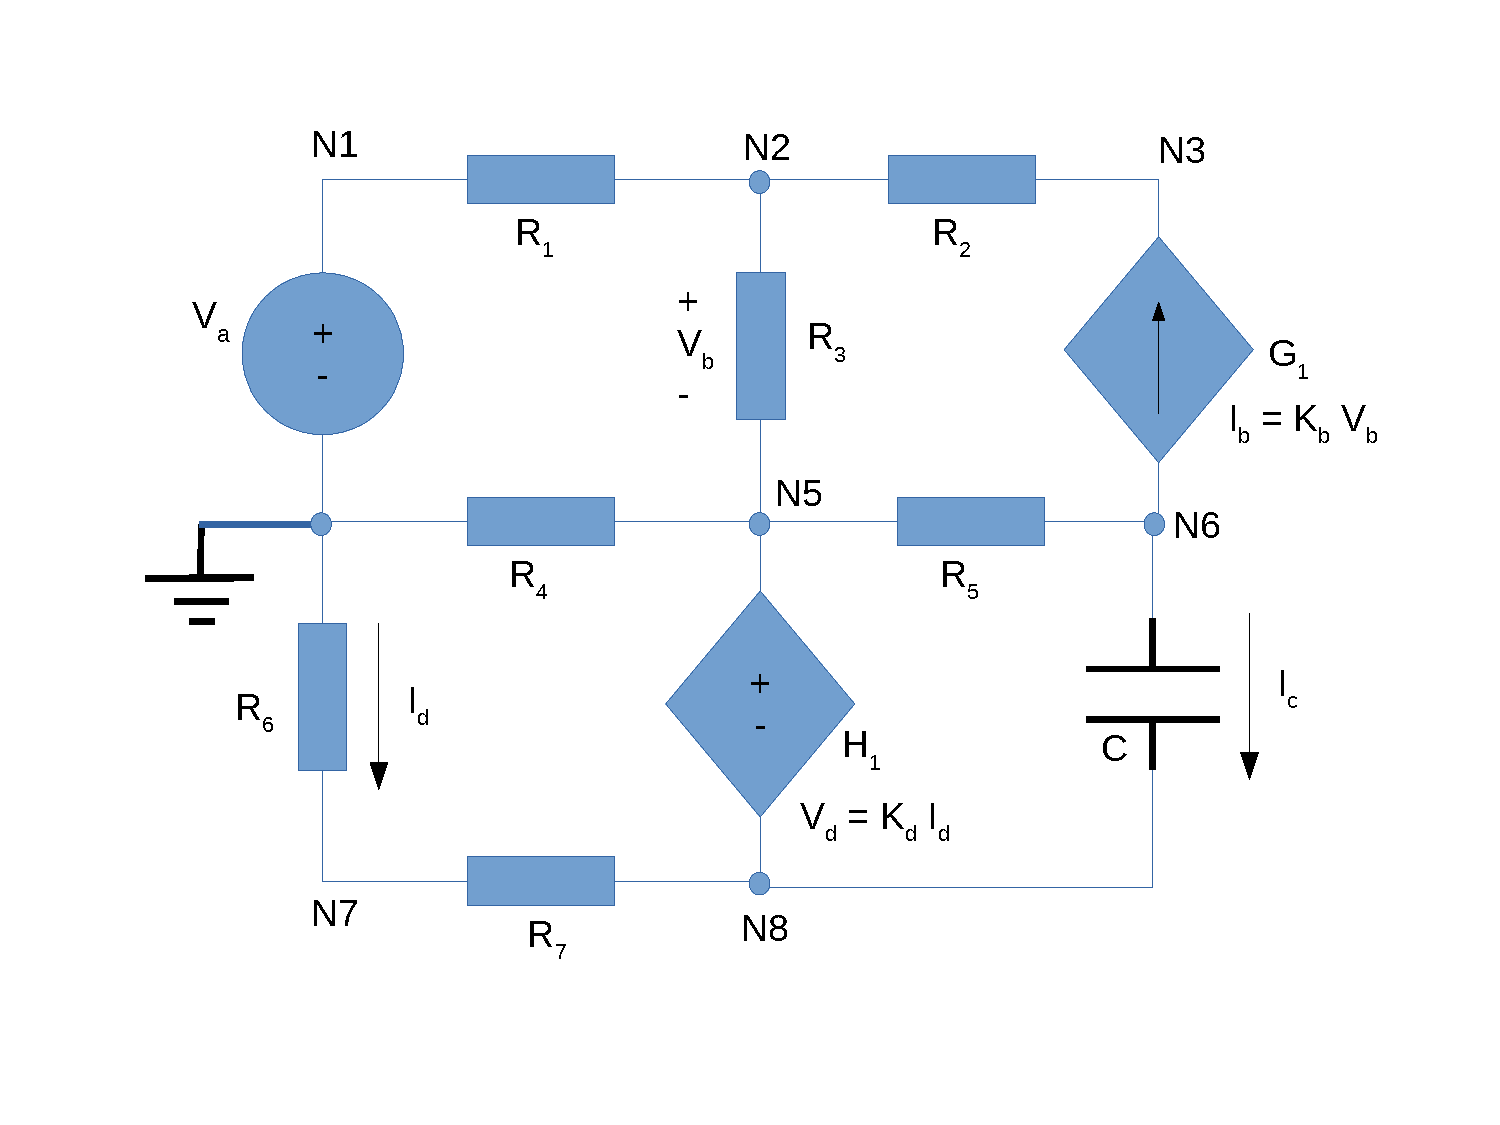
\includegraphics[width=0.85\linewidth]{dsnh_t2.pdf}
	\caption{Circuit T2}
\label{fig:Desenho_t2}
\end{figure}

%-------------------------------------------------------------------------------------------------------
%-------------------------------------------------------------------------------------------------------

\vspace{1cm}

For this laboratory assignment, the values considered for all the varibles can be
found on Table \ref{tab:given_vls}. They were obtained through a Python script that
generates random values. 

\begin{table}[h]
	\centering
	\begin{tabular}{|l|r|}
		\hline    
		{\bf Name} & {\bf Value} \\ \hline
    		%-------------------------------------------------------
% Values from the Python script
% The inserted number was: 95814
%-------------------------------------------------------
% This .tex file was made by hand (non-automaticaly)
%-------------------------------------------------------

$R1$	&	1.00359089673	\\ \hline
$R2$	&	2.04298963569	\\ \hline
$R3$	&	3.02503141993	\\ \hline
$R4$	&	4.05647775356	\\ \hline
$R5$	&	3.07781188185	\\ \hline
$R6$	&	2.01277040929	\\ \hline
$R7$	&	1.01993304256	\\ \hline
$V_a$	&	5.11402517827	\\ \hline
$I_d$	&	1.03896393154	\\ \hline
$K_b$	&	7.23768458527	\\ \hline
$K_c$	&	8.33526265782	\\ \hline

	\end{tabular}
	
	\caption{Values provided by the Python sript. Units for the values: V, mA, kOhm, mS and uF}
    
\label{tab:given_vls}
\end{table}

